\documentclass[12pt,a4paper]{article}
\usepackage{listing}
\usepackage{courier}
\usepackage{ducktex}
\usepackage{float}
\usepackage{graphicx}
\graphicspath{{./images/}}
\floatstyle{boxed} 
\restylefloat{figure}

\author{    
    Jan Neuburger \\
    jan.neuburger.jn@gmail.com
    \and
    Erik Mayrhofer \\
    erik.mayrhofer@liwest.at
    \and
    Florian Schwarcz \\
    florian.schwarcz@gmx.at
    \and
    Maximilian Wahl \\
    mexx.wale@gmail.com
    }
\title{Duckburg\\[0.2em]Troubleshooting Guide}
\begin{document}
\maketitle
\newpage
\tableofcontents
\newpage
\section{Toolignore not working }
\subsection{The error}
If your compile.sh doesn't work or it seems to upload .git or other folders
that are specified in .toolignore, the problem could be the differences between
LF and CRLF.

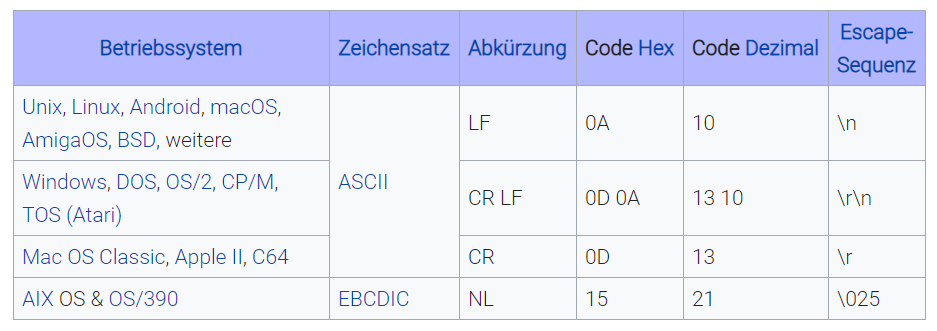
\includegraphics[scale=0.75]{lf_crlf_comparison}

As we can see, LF (used with Unix) uses a different form of line breaks than
CRLF (used under Windows). This causes a problem with the toolignore file so we
have to make shure that all files use LF.
\subsection{Solving the Error}
To solve this problem, Maximilian Wahl has found a short command that you can
simply run in a GitBash or any other Unix Shell.

find . -type f -print0 | xargs -0 dos2unix

It is highly recommended to delete any debug folders created by CMake as the
command would have to iterate over all the files in them and this just takes
too long.
\end{document}